\begin{beginningnote}
    Si tenga presente che alcuni termini utilizzati nel documento riportano la lettera \textbf{G} in apice, allo scopo di evidenziare le parole che assumono uno specifico significato nell'ambito del progetto. Per comprenderle in maniera corretta, si rimanda il lettore al documento ``Glossario", che contiene un elenco completo di tutte le terminologie utilizzate con relative definizioni, allo scopo di costruire un linguaggio uniforme che possa migliorare la comunicazione tra i componenti interni al gruppo e gli stakeholders\textsuperscript{G} esterni.   %inserire corsivo per ogni termine del glossario?
\end{beginningnote}

%%%%%%%%%%%%%%%%%%%%%%%%%%%%%%%%%%%
% SCOPO DEL DOCUMENTO
%%%%%%%%%%%%%%%%%%%%%%%%%%%%%%%%%%%
\section{Scopo del documento}\label{sec:scopo_del_documento}
Questo documento è destinato sia ai membri del gruppo che agli stakeholders in quanto ha come obiettivo quello di indicare tempi, costi e modalità di sviluppo delle varie fasi del progetto\textsuperscript{G}.
In particolare, al suo interno, sono riportati:
\begin{itemize}
    \item Un'analisi dei rischi, comprendente anche delle tecniche di mitigazione implementate per limitarne le problematiche;
    \item Il modello di sviluppo scelto per il progetto;
    \item La pianificazione delle milestones\textsuperscript{G} del progetto, inclusi i relativi costi e tempi di completamento (sia preventivi sia a consuntivo).
\end{itemize}
Vista la natura del documento, è previsto che questo venga redatto in maniera incrementale, aggiornandolo a seconda dei bisogni di gruppo e proponente e in seguito a riflessioni nate dal compimento delle diverse fasi di sviluppo. Per una visione precisa delle modifiche, si rimanda al changelog, che descrive per ciascuna versione le differenze rispetto a quella precedente.

%%%%%%%%%%%%%%%%%%%%%%%%%%%%%%%%%%%
% IL PROGETTO
%%%%%%%%%%%%%%%%%%%%%%%%%%%%%%%%%%%
\section{Il progetto}\label{sec:il_progetto}
\par Il progetto nasce nell'ambito dei \textbf{sistemi gestionali di magazzino}, meglio noti con il termine inglese di \textit{Warehouse Management Systems} (WMS), con l'obiettivo di risolvere una serie di problematiche derivanti dalle soluzioni tradizionali tuttora presenti sul mercato.
\par Il focus principale sarà migliorare la user experience, tramite la realizzazione di un applicativo che proponga all'utente un'interazione con il magazzino in un ambiente di lavoro 3D: questa soluzione, rispetto ai tradizionali sistemi 2D, garantirebbe una maggiore comprensione degli spazi, proponendo una visualizzazione più intuitiva e familiare del magazzino all'utente che, di conseguenza, sarà in grado di prendere decisioni organizzative più informate ed efficienti, ottimizzando i processi di logistica.
\par Per raggiungere questo obiettivo, l'ambiente di lavoro non può essere una semplice visualizzazione del magazzino. L'utente dovrà infatti poter:
\begin{itemize}
    \item Navigare l'ambiente 3D;
    \item Progettare la scaffalatura e modificarla nel tempo;
    \item Simulare i flussi di movimento di mezzi e prodotti.
\end{itemize}
Il progetto deve concretizzarsi nella realizzazione di una web app fruibile agli impiegati d'ufficio ed incentrata sulla visualizzazione 3D del magazzino.
\par Per visionare il capitolato\textsuperscript{G} e la documentazione del gruppo, si veda la sezione \hyperref[sec:riferimenti_esterni]{Riferimenti Esterni} del documento.

\newpage
%%%%%%%%%%%%%%%%%%%%%%%%%%%%%%%%%%%
% ANALISI DEI RISCHI
%%%%%%%%%%%%%%%%%%%%%%%%%%%%%%%%%%%
\section{Analisi dei rischi}\label{sec:analisi_rischi}
Lo scopo di questa sezione è quella di prendere in esame tutte le possibili problematiche che potrebbero verificarsi durante la realizzazione del progetto, al fine di evitare che questi rischi si concretizzino e minaccino così l'avanzamento delle attività di progetto.
Questa analisi sarà organizzata in forma tabellare, in modo da consentire un monitoraggio continuo e più accessibile, e dividendo i rischi a seconda delle seguenti categorie:
\begin{itemize}
    \item Rischi di tipo tecnico-tecnologico;
    \item Rischi organizzativi.
\end{itemize}
In particolare, per ciascun rischio viene fornito:
\begin{itemize}
    \item \textbf{Una breve descrizione}.
    \item \textbf{La probabilità di occorrenza}, indicata attraverso:
        \begin{itemize}
            \item \textbf{A}: per occorrenza alta;
            \item \textbf{M}: per occorrenza media;
            \item \textbf{B}: per occorrenza bassa.
        \end{itemize}
    \item \textbf{Il grado di pericolosità}, indicato attraverso i seguenti colori:
        \begin{itemize}
        \item \colorbox{red!50}{\textbf{Rosso:}} per rischi con pericolosità alta;
        \item \colorbox{orange!50}{\textbf{Arancione:}} per rischi con pericolosità media;
        \item \colorbox{yellow!75}{\textbf{Giallo:}} per rischi con pericolosità bassa.
        \end{itemize}
    \item \textbf{Precauzioni da prendere}.
    \item \textbf{Il piano di contingenza}\textsuperscript{G}.
\end{itemize}

\subsection{Rischi di tipo tecnico-tecnologico}\label{sec:analisi_rischi:tec}
\renewcommand{\arraystretch}{1.5}
\begin{xltabular}{\textwidth}{p{0.00001\textwidth} X | X | X | p{0.05\textwidth}}
    \rowcolor{black}
    & \textbf{\color{white} Rischio} & \textbf{\color{white} Precauzioni} & \textbf{\color{white} Piano di contingenza} & \textbf{\color{white} Occ.}\\ 
    \hline
    \endhead
    
    \cellcolor{red}& \textbf{Tecnologie sconosciute:} il gruppo ha scarsa esperienza con le tecnologie da utilizzare in fase di codifica del prodotto software. 
    & Ogni membro deve comunicare ai colleghi il suo livello di conoscenza relativo alla tecnologia da utilizzare per migliorare l'efficienza del gruppo (e.g. trovando una migliore suddivisione del lavoro).
    & Si cerca di approfondire la tecnologia da utilizzare con lo studio individuale, ed eventualmente collettivo, della documentazione fornita. Nel caso la tecnologia non sia funzionale e/o causi ritardi troppo prolungati si può valutarne la sostituzione o dismissione. 
    & A \\
    \hline
    
    \cellcolor{orange}& \textbf{Strumenti sconosciuti:} il gruppo non ha alcuna esperienza con software di gestione dei progetti. 
    & Prima di utilizzare uno strumento sconosciuto, si valuta congiuntamente l'efficienza/efficacia del suo utilizzo. Ogni membro dovrà poi esercitarsi a comprendere gli aspetti principali dello strumento e segnalare le eventuali difficoltà incontrate.
    & In caso di dubbi non risolti attraverso lo studio individuale, si può ricorrere ad un incontro con altri membri del gruppo per cercare di risolvere il problema più velocemente. Altrimenti, se ciò è causa di ritardi troppo lunghi, si cerca un'alternativa o si valuta di non usarlo. 
    & A \\
    \hline

    \cellcolor{orange}& \textbf{Problemi hardware o software:} lo strumento di lavoro (sia esso software o hardware) di un componente del gruppo potrebbe non permettere, totalmente o parzialmente, lo svolgimento di una qualche attività del progetto. 
    & Il membro che incorrerà in questo rischio (e.g. a causa di un guasto) dovrà farlo presente tempestivamente agli altri membri del gruppo.
    & Si cerca di utilizzare software affidabili ed effettuare backup periodici. Nel caso di malfunzionamento del dispositivo, è necessario cercare di svolgere i compiti assegnati usandone un altro. Se ciò non fosse possibile, si cerca di ridistribuire le attività in modo da limitare il più possibile il risultante rallentamento nello sviluppo del progetto.
    & B \\
    \hline \\

    \caption{Tabella dei rischi di tipo tecnico-tecnologico}
    \label{tab:rischi:tec}
\end{xltabular}

\subsection{Rischi organizzativi}\label{sec:analisi_rischi:org}
\renewcommand{\arraystretch}{1.5}
\begin{xltabular}{\textwidth}{p{0.00001\textwidth} X | X | X | p{0.05\textwidth}}

    \rowcolor{black}
    & \textbf{\color{white} Rischio} & \textbf{\color{white} Precauzioni} & \textbf{\color{white} Piano di contingenza} & \textbf{\color{white} Occ.}\\ 
    \hline
    \endhead
    
    \cellcolor{red}& \textbf{Inesperienza professionale-organizzativa:} la maggior parte del gruppo affronta per la prima volta un progetto così complesso.
    & Ogni membro deve comunicare ai colleghi quelli che potrebbero rivelarsi dei punti di criticità.
    & Si cerca di approfondire quanto possibile con lo studio individuale. Se ciò non dovesse bastare, il membro può richiedere un aiuto agli altri componenti del gruppo. Nel caso la criticità persistesse, si richiedono chiarimenti ai docenti del corso e/o all'azienda proponente.
    & A \\
    \hline

    \cellcolor{red}& \textbf{Prospetti economici e temporali non rispettati: } i costi monetari e temporali per le varie attività potrebbero essere stati stimati incorrettamente a causa dell'inesperienza del gruppo in tal senso.
    & Si cerca di non pianificare in maniera ottimistica ma tenendo presente eventuali ostacoli in cui si potrebbe incorrere durante l'avanzamento del progetto. Per quanto riguarda la gestione delle scadenze, il responsabile si impegna a richiamare l'attenzione del gruppo su quelle imminenti per evitare slittamenti nel progetto.
    & Se un membro del gruppo si accorge che non sta rispettando la pianificazione lo farà presente al responsabile, che valuterà una rilocazione di risorse oppure, in casi estremi, la modifica del preventivo proposto.
    & A \\
    \hline
    
    \cellcolor{orange}& \textbf{Disponibilità oraria varia:} i membri del gruppo hanno impegni diversi che potrebbero generare difficoltà nelle tempistiche di lavoro e/o nell'organizzazione di incontri collettivi.
    & Ogni membro si impegna ad essere il più possibile reperibile e, se ciò non fosse possibile, di comunicare le sue disponibilità agli altri membri in modo da poter organizzare il lavoro in maniera più efficiente.
    & Si comunica agli altri membri del gruppo i propri impegni attraverso gli strumenti predisposti e si cerca di trovare assieme una soluzione che sfrutti al meglio il tempo a disposizione di tutti.
    & M \\
    \hline

    \cellcolor{yellow}& \textbf{Comunicazione esterna:} una parte del gruppo non ha conoscenza pratica per quanto riguarda la comunicazione in ambito professionale.
    & Il gruppo affida al proponente esterno, più esperto, la scelta del canale di comunicazione più appropriato.
    & Il gruppo si impegna a seguire le indicazioni fornite dal proponente in merito. Altrimenti, si cerca, assieme ai membri più esperti, di pensare a soluzioni alternative da proporre.
    & M \\
    \hline

    \cellcolor{red}& \textbf{Modifiche al progetto in corso d'opera:} l'azienda potrebbe richiedere l'aggiunta e/o modifica di alcuni requisiti, tecnologie e funzionalità a progetto già iniziato.
    & Il gruppo aggiorna l'azienda al completamento di ogni obiettivo prestabilito in modo che questa possa valutare attentamente il lavoro svolto.
    & Si mantiene un rapporto continuativo con l'azienda, aggiornandola sull'avanzamento del progetto. Se l'azienda dovesse comunicare al gruppo un cambiamento, le attività saranno ristrutturate dal responsabile di conseguenza.
    & B \\
    \hline

    \cellcolor{orange}& \textbf{Rapporti interni:} si potrebbero verificare delle difficoltà qualora due o più membri del gruppo dovessero trovarsi, per un qualche motivo, in disaccordo sulle decisioni da prendere.
    & Si cerca di evitare queste situazioni e pensare in ottica collettiva, cercando compromessi.
    & Le opinioni di tutti devono essere discusse allo scopo di prendere la decisione migliore. Nel caso di conflitti, è nell'interesse di tutti i membri del gruppo reinstaurare e mantenere un dialogo costruttivo.
    & B \\
    \hline

    \cellcolor{orange}& \textbf{Distribuzione disomogenea:} il carico di lavoro potrebbe essere mal distribuito, e.g. troppo dispendioso per alcuni e/o troppo leggero per altri. 
    & Ciascun membro, in base alle proprie disponibilità e agli impegni presi per il progetto, si impegna a far presente al gruppo le proprie capacità, segnalando eventuali compiti che potrebbero essere non/più adatti alla sua situazione corrente e futura.
    & Sarà compito del responsabile decidere come redistribuire il lavoro in maniera più efficiente.
    & B \\
    \hline

    \cellcolor{orange}& \textbf{Rapporti esterni: } il proponente potrebbe essere poco presente e/o di scarso aiuto.
    & Si cerca di capire fin da subito le disponibilità dell'azienda.
    & Il responsabile si occuperà di gestire la comunicazione esterna cercando di far presente se dovessero esserci delle difficoltà in tal senso.
    & B \\
    \hline \\

    \caption{Tabella dei rischi organizzativi}
    \label{tab:rischi:org}
\end{xltabular}

\newpage
%%%%%%%%%%%%%%%%%%%%%%%%%%%%%%%%%%%
% MODELLO DI SVILUPPO
%%%%%%%%%%%%%%%%%%%%%%%%%%%%%%%%%%%
\section{Modello di sviluppo}\label{sec:modello_sviluppo}
Un modello di ciclo di vita\textsuperscript{G} serve a fornire relazioni temporali e logiche di un processo software.
Noi di Avant-Garde abbiamo deciso di adottare un modello di vita iterativo, più precisamente un modello agile.
% Illustrare e spiegare la scelta del modello di sviluppo da applicare al progetto

\subsection{Il modello agile}\label{sec:modello_sviluppo:agile}
La metodologia Agile è un approccio alla gestione dei progetti che prevede la suddivisione del progetto in fasi e sottolinea l'importanza della collaborazione e del miglioramento continui, tramite frequenti incontri tra i membri del gruppo e con l'azienda.
I vantaggi di un modello agile comprendono:
\begin{itemize}
    \item Rispondere in modo rapido e flessibile alle richieste dei clienti;
    \item Alta comunicazione fra sviluppatori e cliente;
    \item Diverse fasi che permettono i vantaggi di un modello incrementale.
\end{itemize}
Un ciclo di vita di un modello agile si divide in 5 fasi:
    \subsubsection{Envision}\label{sec:modello_sviluppo:agile:envision}
    Fase in cui si determinano con il cliente gli obiettivi del progetto, si decide il team e le norme da utilizzare.
    Alla fine della fase di Envision si ha:
    \begin{itemize}
        \item Un Piano di Progetto che ne descriva lo scopo;
        \item Gli obiettivi complessivi del progetto;
        \item Gli stakeholder del progetto;
        \item Strumenti di collaborazione del gruppo funzionanti.
    \end{itemize}
    Una volta terminata la fase di Envision, si passa per ogni sprint attraverso le prossime tre fasi: Speculate, Explore e Adapt.
    \subsubsection{Speculate}\label{sec:modello_sviluppo:agile:speculate}
    La fase Speculate è un esercizio di pianificazione. Durante questa fase, si sviluppa o rivede il piano di consegna basato sulle feature\textsuperscript{G}, le stime per ogni feature, e i rischi da gestire. In ogni sprint vengono completate una o più feature. %Una feature è un pezzo di funzionalità o outcome che ha valore per il cliente.
    La fase di Speculate termina quando sono definiti una serie di requisiti per lo sprint e una lista di feature da sviluppare in base ai requisiti. Inoltre si ha una stima del lavoro necessario per ogni feature, e i rischi verranno identificati o aggiornati per le feature su cui si sta lavorando.
    \subsubsection{Explore}\label{sec:modello_sviluppo:agile:explore}
    Durante la fase Explore si sviluppa effettivamente il prodotto. Sono previsti incontri frequenti tra i membri del gruppo e revisioni delle feature non appena vengono create.
    \subsubsection{Adapt}\label{sec:modello_sviluppo:agile:adapt}
    La fase di Adapt consiste in una revisione finale delle feature da parte del cliente e una riunione documentata dei membri del team per riflettere su ciò che è stato fatto. Si condivide l'esperienza accumulata nel corso di progetto e viene rivista la pianificazione per lo sprint successivo.
    \subsubsection{Close}\label{sec:modello_sviluppo:agile:close}
    Il progetto passa per le fasi di speculate, explore e adapt fino al momento in cui tutti gli sprint per il progetto sono completati. Una volta finite tutte le iterazioni e implementate le feature, arriva la fase Close, di chiusura.
    Durante questa fase ci si assicura che i deliverable\textsuperscript{G} siano completati.

\subsection{Incrememnti individuati}\label{sec:modello_sviluppo:incrementi}
Per comodità di esposizione, in questo documento le fasi di Speculate, Explore e Adapt saranno raggruppate in un singolo periodo di tempo chiamato ``incremento".
Gli incrementi individuati sono 4 e fanno riferimento al periodo antecedente la prima revisione (Requirements and Technology Baseline).
La tabella sarà soggetta a cambiamenti derivati dai futuri incrememnti.
\begin{xltabular}{\textwidth}{p{0.05\textwidth} | p{0.5\textwidth} }

    \rowcolor{black}
    \textbf{\color{white} Incr.} & \textbf{\color{white} Obiettivi} \ 
    \hline
    \endhead
    
    \textbf{I} 
    & \textbf{Visualizzazione ambiente 3d:} Prima di tutto, è necessario potersi muovere all'interno dello spazio 3D e creare un magazzino partendo dalle sue dimensioni. \\
    \hline

    \textbf{II} 
    & \textbf{Creazione e aggiunta scaffalature:} Una volta creato l'ambiente, è necessario poter creare delle nuove scaffalature e inserirle all'interno del magazzino. \\
    \hline

    \textbf{III} 
    & \textbf{Implementazione item:} Dopo l'implementazione delle scaffalature, si può passare all'introduzione degli item (dei prodotti) all'interno di esse. \\
    \hline

    \textbf{IV} 
    & \textbf{Creazione richieste spostamento:} Possibilità di creare una richiesta di spostamento di un item da un luogo all'altro del magazzino. \\
    \hline

\caption{Tabella degli incrementi individuati}\label{tab:incrementi}
\end{xltabular}

\newpage
%%%%%%%%%%%%%%%%%%%%%%%%%%%%%%%%%%%
% PIANIFICAZIONE
%%%%%%%%%%%%%%%%%%%%%%%%%%%%%%%%%%%
\section{Pianificazione}\label{sec:pianificazione}

La pianificazione è stata suddivisa nelle seguenti cinque fasi:

\begin{itemize}
    \item Analisi
    \item Progettazione della Technology Baseline
    \item Codifica della Technology Baseline
    \item Progettazione dettaglio e codifica finale
    \item Validazione e collaudo
\end{itemize}

Ogni attività può essere suddivisa in ulteriori sottoperiodi con obiettivi più specifici. Ciascun sottoperiodo riporta una tabella con obiettivi e descrizione e ad ogni fase è associato un diagramma di Gantt che riporta le tempistiche previste.

\subsection{Analisi}\label{sec:pianificazione:analisi}

\textbf{Periodo}: dal 06/11/2023 al 06/01/2024\\\\
Questa fase inzia dopo l'assegnazione del capitolato d'appalto e termina il 06/01/2024 come concordato dal gruppo. Gli obiettivi di questa fase, che corrisponde al momento di \textit{Envision} nel modello agile, sono l'analisi in dettaglio del capitolato \textit{Warehouse Management Systems} (WMS), individuando i requisiti di progetto, e il completamento della stesura dei documenti preliminari alla codifica.

\subsubsection{Attività}\label{sec:pianificazione:analisi:attivita}
\begin{itemize}
    \item \textbf{Norme di progetto:} stesura del documento \textit{Norme di progetto} necessario a descrivere le regole che il gruppo si impone per il corretto svolgimento del progetto. Con la stesura del documento vengono inoltre studiate le tecnologie e gli strumenti che verranno utilizzati nella stesura dei documenti e nel progetto.
    \item \textbf{Piano di progetto:} stesura del documento \textit{Piano di progetto}, che presenta un'analisi dei rischi, descrive il piano di progetto in dettaglio e il calcolo del preventivo per la realizzazione del progetto.
    \item \textbf{Piano di qualifica:} stesura del documento \textit{Piano di qualifica}, in cui vengono esposte tecniche e metodi utilizzati per garantire la qualità del prodotto.
    \item \textbf{Analisi dei requisiti:} stesura del documento di \textit{Analisi dei requisiti}, con una descrizione approfondita dei casi d'uso per il prodotto software e dei requisiti di progetto emersi dallo studio del capitolato, dei casi d'uso stessi e attraverso gli incontri con il proponente.
    \item \textbf{Glossario:} stesura del \textit{Glossario}, che dovrà contenere i termini principali utilizzati nell'ambito del progetto.
\end{itemize}


\subsubsection{Periodi}\label{sec:pianificazione:analisi:periodi}
Questa fase è suddivisa in tre periodi come descritto nelle pagine successive.

\newpage

\paragraph{Primo periodo}\label{sec:pianificazione:analisi:periodi:primo}

\begin{xltabular}{\textwidth}{{0.35\textwidth} | X}
        
    \rowcolor{black}
    \textbf{\color{white} Info} & \textbf{\color{white} Primo Periodo}\\ 
    \hline
    \endhead
    
    \textbf{Data inizio} 
    & 12/11/2023 \\
    \hline

    \textbf{Data fine} 
    & 30/11/2023 \\
    \hline

    \textbf{Pre-condizione} 
    & Assegnazione del capitolato \\
    \hline
    
    \textbf{Post-condizione} 
    & Stesura iniziale dei documenti elencati attraverso l'utilizzo dei nuovi mezzi e del template crato appositamente \\
    \hline

    \textbf{Ruoli attivi} 
    &  \begin{itemize}
        \item Responsabile
        \item Amministratore
        \item Verificatore
        \item Analista
    \end{itemize}\\
    \hline

    \textbf{Descrizione} 
    &  Il gruppo effettua un'analisi preliminare del progetto, anche confrontandosi con l'azienda, e comincia il lavoro di stesura dei documenti che verranno presentati alla revisione della Technology Baseline, a partire dallo studio degli strumenti che verranno utilizzati. \\
    \hline
    
    \textbf{Attività} 
    & \begin{itemize}
        \item Individuazione e studio strumenti
        \item Stesura documento \textit{Norme di progetto} con i dettagli sui metodi di svolgimento del progetto e descrizione degli strumenti che verranno utilizzati
        \item Inizio stesura documento \textit{Piano di progetto}
        \item Inizio stesura documento \textit{Piano di qualifica}
        \item Inizio del lavoro di analisi dei requisiti e incontri con il proponente
        \item Stesura del glossario
    \end{itemize} \\
    \hline

\caption{Tabella descrittiva del periodo 1 della fase di analisi}\label{tab:periodo1_1}
\end{xltabular}

\newpage
\paragraph{Secondo periodo}\label{sec:pianificazione:analisi:periodi:secondo}

\begin{xltabular}{\textwidth}{{0.35\textwidth} | X}
        
    \rowcolor{black}
    \textbf{\color{white} Info} & \textbf{\color{white} Secondo Periodo}\\ 
    \hline
    \endhead
    
    \textbf{Data inizio} 
    & 31/11/2023 \\
    \hline

    \textbf{Data fine} 
    & 02/01/2024 \\
    \hline

    \textbf{Pre-condizione} 
    & Soddisfacimento post-condizioni del periodo precedente \\
    \hline
    
    \textbf{Post-condizione} 
    & Completamento della stesura dei documenti iniziati durante la fase precedente \\
    \hline

    \textbf{Ruoli attivi} 
    &  \begin{itemize}
        \item Responsabile
        \item Amministratore
        \item Verificatore
        \item Analista
    \end{itemize}\\
    \hline

    \textbf{Descrizione} 
    &  Il gruppo si impegna a continuare e completare i documenti iniziati durante la fase precedente in vista della verifica e approvazione di questi. Il documento \textit{Norme di progetto} è completato e deve essere perfezionato. \\
    \hline
    
    \textbf{Attività} 
    & \begin{itemize}
        \item Perfezionamento del documento \textit{Norme di progetto}, verifica e approvazione dello stesso
        \item Completamento stesura documento \textit{Piano di progetto}
        \item Completamento stesura documento \textit{Piano di qualifica}
        \item Completamento del lavoro di analisi dei requisiti e stesura dell'omonimo documento
        \item Aggiornamento del glossario con i nuovi termini individuati dalla documentazione
    \end{itemize} \\
    \hline

\caption{Tabella descrittiva del periodo 2 della fase di analisi}\label{tab:periodo1_2}
\end{xltabular}

\newpage
\paragraph{Terzo periodo}\label{sec:pianificazione:analisi:periodi:terzo}

\begin{xltabular}{\textwidth}{{0.35\textwidth} | X}
        
    \rowcolor{black}
    \textbf{\color{white} Info} & \textbf{\color{white} Terzo Periodo}\\ 
    \hline
    \endhead
    
    \textbf{Data inizio} 
    & 03/01/2024 \\
    \hline

    \textbf{Data fine} 
    & 06/01/2024 \\
    \hline

    \textbf{Pre-condizione} 
    & Soddisfacimento post-condizioni del periodo precedente \\
    \hline
    
    \textbf{Post-condizione} 
    & Verifica e approvazione di tutti i documenti prodotti nella fase corrente. \\
    \hline

    \textbf{Ruoli attivi} 
    &  \begin{itemize}
        \item Responsabile
        \item Amministratore
        \item Verificatore
        \item Analista
    \end{itemize}\\
    \hline

    \textbf{Descrizione} 
    &  I documenti scritti vengono ora verificati e approvati secondo quanto stabilito nel \textit{Piano di qualifica}, accertandosi che tutti seguano quanto stabilito nelle \textit{Norme di progetto}. \\
    \hline
    
    \textbf{Attività} 
    & \begin{itemize}
        \item Perfezionamento del documento \textit{Norme di progetto}, verifica e approvazione dello stesso
        \item Verifica e approvazione del documento \textit{Piano di progetto}
        \item Verifica e approvazione del documento \textit{Piano di qualifica}
        \item Verifica e approvazione del documento \textit{Analisi dei requisiti}
        \item Verifica e aggiornamento del glossario
    \end{itemize} \\
    \hline

\caption{Tabella descrittiva del periodo 3 della fase di analisi}\label{tab:periodo1_3}
\end{xltabular}

\newpage 
\subsubsection{Diagramma di Gantt}\label{sec:pianificazione:analisi:gantt}

\begin{figure}[H]
    \centering
    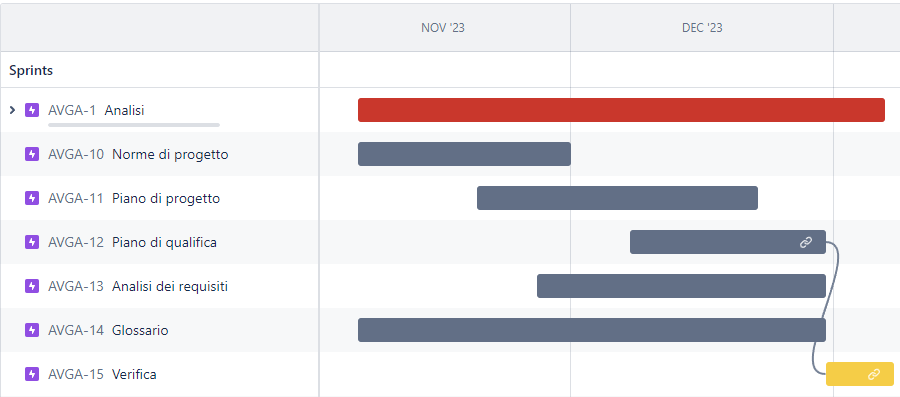
\includegraphics[width=1\textwidth]{images/gantt_analisi.PNG}
    \caption{Diagramma di Gantt della fase di analisi}
    \label{fig:gantt_analisi}
\end{figure}

%%%%%%%%%%%%%%%%%%%%%%%%%%%%%%%%%%%   PROGETTAZIONE RTB   %%%%%%%%%%%%%%%%%%%%%%%%%%%%%%%%%%%

\subsection{Progettazione della Technology Baseline}\label{sec:pianificazione:progRTB}

\textbf{Periodo}: dal 07/01/2024 al 23/02/2024\\\\
Questa fase inizia una volta completati tutti i documenti preliminari previsti nella fase di Analisi e termina il 23/02/2024 come concordato dal gruppo, con il completamento della codifica del \textit{Proof of concept}\textsuperscript{G} (abbreviato in \textit{PoC}). Al termine della fase il gruppo avr`a creato un PoC funzionante che verr`a presentato alla revisione della Technology Baseline.

\subsubsection{Attività}\label{sec:pianificazione:progRTB:attivita}
\begin{itemize}
    \item \textbf{Studio tecnologie:} Studio delle tecnologie nuove al gruppo per l'implementazione del Proof of Concept.
    \item \textbf{Progettazione PoC:} Progettazione del Proof of Concept e discussione con l'azienda.
    \item \textbf{Codifica PoC:} Codifica del Proof of Concept.
    \item \textbf{Aggiornamento documentazione:} Ulteriore revisione dei documenti ed eventuale aggiornamento di essi.
\end{itemize}

\subsubsection{Periodi}\label{sec:pianificazione:progRTB:periodi}
Questa fase è composta da un periodo di progettazione seguita da 4 sprint di avanzamento della codifica del Proof of Concept.

\newpage

\paragraph{Primo periodo}\label{sec:pianificazione:progRTB:periodi:primo}

\begin{xltabular}{\textwidth}{{0.35\textwidth} | X}
        
    \rowcolor{black}
    \textbf{\color{white} Info} & \textbf{\color{white} Primo Periodo}\\ 
    \hline
    \endhead
    
    \textbf{Data inizio} 
    & 07/01/2024 \\
    \hline

    \textbf{Data fine} 
    & 15/01/2024 \\
    \hline

    \textbf{Pre-condizione} 
    & Soddisfacimento post-condizioni del periodo precedente \\
    \hline
    
    \textbf{Post-condizione} 
    & Lo studio delle tecnologie adottate per la codifica è terminato e la progettazione architetturale minimale del PoC è definita. \\
    \hline

    \textbf{Ruoli attivi} 
    &  \begin{itemize}
        \item Responsabile
        \item Amministratore
        \item Verificatore
        \item Analista
        \item Progettista
    \end{itemize}\\
    \hline

    \textbf{Descrizione} 
    &  Durante questo periodo si lavora sulla progettazione del Proof of Concept, ad un livello minimale e non eccessivamente approfondito vista la natura ``usa e getta" del PoC, si prende familiarità con le tecnologie necessarie e si discute con l'azienda sui requisiti minimi da implementare all'interno del PoC. Si effettuano eventuali modifiche e correzioni dei documenti. \\
    \hline
    
    \textbf{Attività} 
    & \begin{itemize}
        \item Studio tecnologie per la codifica del PoC 
        \item Riunioni con l'azienda per discutere dei requisiti minimi da implementare nel PoC
        \item Aggiornamento dei documenti
    \end{itemize} \\
    \hline

\caption{Tabella descrittiva del periodo 1 della fase di progettazione della Technology Baseline}\label{tab:periodo2_1}
\end{xltabular}

\newpage 

\paragraph{Primo sprint}\label{sec:pianificazione:codificaRTB:periodi:primo}

\begin{xltabular}{\textwidth}{{0.35\textwidth} | X}
        
    \rowcolor{black}
    \textbf{\color{white} Info} & \textbf{\color{white} Primo sprint}\\ 
    \hline
    \endhead
    
    \textbf{Data inizio} 
    & 16/01/2024 \\
    \hline

    \textbf{Data fine} 
    & 21/01/2024 \\
    \hline

    \textbf{Pre-condizione} 
    & Soddisfacimento post-condizioni del periodo precedente. \\
    \hline
    
    \textbf{Post-condizione} 
    & Interfaccia utente che permette di visualizzare un ambiente 3D. \\
    \hline

    \textbf{Ruoli attivi} 
    &  \begin{itemize}
        \item Responsabile
        \item Amministratore
        \item Verificatore
        \item Progettista
        \item Programmatore
    \end{itemize}\\
    \hline
    
    \textbf{Attività} 
    & \begin{itemize}
        \item Approfondimento delle tecnologie studiate finora 
        \item \textbf{Creazione ambiente 3D:} Implementazione di un'interfaccia utente che permetta di muoversi all'interno di un ambiente 3D che visualizza un magazzino con dimensioni inserite dall'utente
    \end{itemize} \\
    \hline

\caption{Primo sprint PoC}\label{tab:periodo3_1}
\end{xltabular}

\newpage
\paragraph{Secondo sprint}\label{sec:pianificazione:codificaRTB:periodi:secondo}

\begin{xltabular}{\textwidth}{{0.35\textwidth} | X}
        
    \rowcolor{black}
    \textbf{\color{white} Info} & \textbf{\color{white} Secondo sprint}\\ 
    \hline
    \endhead
    
    \textbf{Data inizio} 
    & 22/01/2024 \\
    \hline

    \textbf{Data fine} 
    & 04/02/2024 \\
    \hline

    \textbf{Pre-condizione} 
    & Soddisfacimento post-condizioni dello sprint precedente. \\
    \hline
    
    \textbf{Post-condizione} 
    & Possibilità di creare, modificare, piazzare e muovere scaffalature. \\
    \hline

    \textbf{Ruoli attivi} 
    &  \begin{itemize}
        \item Responsabile
        \item Amministratore
        \item Verificatore
        \item Programmatore
    \end{itemize}\\
    \hline
    
    \textbf{Attività} 
    & \begin{itemize}
        \item \textbf{Creazione scaffalature:} Implementazione della funzionalità che permetta all'utente di creare una nuova scaffalatura
        \item \textbf{Piazzamento scaffalature:} Possibilità di poter piazzare la scaffalatura creata all'interno del magazzino 3D
        \item \textbf{Spostamento scaffalature:} Possibilità di spostare, modificare o eliminare una scaffalatura piazzata in precedenza nel magazzino 3D
    \end{itemize} \\
    \hline

\caption{Secondo sprint PoC}\label{tab:periodo3_2}
\end{xltabular}
\newpage
\paragraph{Terzo sprint}\label{sec:pianificazione:codificaRTB:periodi:terzo}

\begin{xltabular}{\textwidth}{{0.35\textwidth} | X}
        
    \rowcolor{black}
    \textbf{\color{white} Info} & \textbf{\color{white} Terzo sprint}\\ 
    \hline
    \endhead
    
    \textbf{Data inizio} 
    & 05/02/2024 \\
    \hline

    \textbf{Data fine} 
    & 15/02/2024 \\
    \hline

    \textbf{Pre-condizione} 
    & Soddisfacimento post-condizioni dello sprint precedente. \\
    \hline
    
    \textbf{Post-condizione} 
    & Aggiunta di prodotti con possibilità di piazzarli nelle scaffalature presenti nel magazzino 3D. \\
    \hline

    \textbf{Ruoli attivi} 
    &  \begin{itemize}
        \item Responsabile
        \item Amministratore
        \item Verificatore
        \item Programmatore
    \end{itemize}\\
    \hline
    
    \textbf{Attività} 
    & \begin{itemize}
        \item \textbf{Creazione prodotto:} Tramite interfaccia utente, possibilità di creare un nuovo prodotto
        \item \textbf{Posizionamento prodotto:} Possibilità di piazzare il prodotto creato all'interno di una scaffalatura libera
    \end{itemize} \\
    \hline

\caption{Terzo sprint PoC}\label{tab:periodo3_3}
\end{xltabular}

\newpage
\paragraph{Quarto sprint}\label{sec:pianificazione:codificaRTB:periodi:quarto}

\begin{xltabular}{\textwidth}{{0.35\textwidth} | X}
        
    \rowcolor{black}
    \textbf{\color{white} Info} & \textbf{\color{white} Quarto sprint}\\ 
    \hline
    \endhead
    
    \textbf{Data inizio} 
    & 16/01/2024 \\
    \hline

    \textbf{Data fine} 
    & 23/02/2024 \\
    \hline

    \textbf{Pre-condizione} 
    & Soddisfacimento post-condizioni dello sprint precedente. \\
    \hline
    
    \textbf{Post-condizione} 
    & Possibilità di creare una richiesta di spostamento di un item da un luogo ad un altro. \\
    \hline

    \textbf{Ruoli attivi} 
    &  \begin{itemize}
        \item Responsabile
        \item Amministratore
        \item Verificatore
        \item Programmatore
    \end{itemize}\\
    \hline
    
    \textbf{Attività} 
    & \begin{itemize}
        \item \textbf{Interfaccia spostamento oggetto:} Creazione di un'interfaccia che permetta di creare una richiesta di spostamento di un prodotto da un luogo ad un altro
        \item \textbf{Creazione richiesta spostamento:} implementare la creazione di una richiesta di spostamento di un prodotto
    \end{itemize} \\
    \hline

\caption{Quarto sprint PoC}\label{tab:periodo3_4}
\end{xltabular}

\newpage 
\subsubsection{Diagramma di Gantt}\label{sec:pianificazione:codificaRTB:gantt}

\begin{figure}[H]
    \centering
    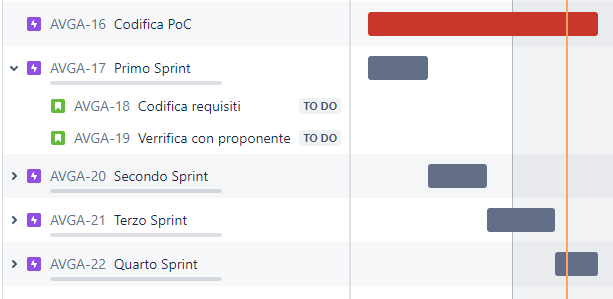
\includegraphics[width=0.75\textwidth]{images/gantt_codRTB.PNG}
    \caption{Diagramma di Gantt della fase di codifica del PoC}
    \label{fig:gantt_codRTB}
\end{figure}

%%%%%%%%%%%%%%%%%%%%%%%%%%%%%%%%%%%   PROGETTAZIONE E CODIFICA   %%%%%%%%%%%%%%%%%%%%%%%%%%%%%%%%%%%

\subsection{Progettazione di dettaglio e codifica finale}\label{sec:pianificazione:progCodifica}

\textbf{Periodo}: dal 24/02/2024 al 01/04/2024\\\\
Questa fase inizia una volta completata la codifica del \textit{Proof of Concept} e completata la prima revisione. La fase termina il 01/04/2024 come concordato dal gruppo, con un prodotto funzionante e pronto per la consegna al proponente. Durante questa fase verranno anche creati documenti quali il \textit{Manuale Utente}, il \textit{Manuale del Manutentore} e l'\textit{Allegato Tecnico}.


\subsubsection{Attività}\label{sec:pianificazione:prog_codifica:attivita}
\begin{itemize}
    \item \textbf{Progettazione di dettaglio:} Viene progettato nel dettaglio il prodotto finale, in modo da poterlo implementare in modo efficiente, completo e con meno problematiche possibile. 
    \item \textbf{Incremento dei documenti:} Aggiornamento e verifica dei documenti.
    \item \textbf{Codifica:} Viene implementato il prodotto finale, partendo da quanto emerso tramite la realizzazione del PoC. La codifica avviene in modo incrementale, seguendo gli incrementi individuati nella fase di analisi secondo il modello Agile.
    \item \textbf{Manuale Utente:} Stesura del Manuale Utente.
    \item \textbf{Manuale del Manutentore:} Stesura del Manuale del Manutentore.
    \item \textbf{Allegato Tecnico:} Stesura dell'Allegato Tecnico.
    \item \textbf{Product Baseline:} Realizzazione dei diagrammi di sequenza e di attività.
    \item \textbf{Verifica:} Il codice viene verificato in fase di scrittura per facilitare il lavoro nella fase di validazione.
\end{itemize}

\subsubsection{Periodi}\label{sec:pianificazione:prog_codifica:periodi}
Questa fase è suddivisa in due periodi come descritto nelle pagine successive.

\newpage

\paragraph{Primo periodo}\label{sec:pianificazione:prog_codifica:periodi:primo}

\begin{xltabular}{\textwidth}{{0.35\textwidth} | X}
        
    \rowcolor{black}
    \textbf{\color{white} Info} & \textbf{\color{white} Primo Periodo}\\ 
    \hline
    \endhead
    
    \textbf{Data inizio} 
    & 25/02/2024 \\
    \hline

    \textbf{Data fine} 
    & 05/03/2024 \\
    \hline

    \textbf{Pre-condizione} 
    & Soddisfacimento post-condizioni del periodo precedente, revisione del RTB. \\
    \hline
    
    \textbf{Post-condizione} 
    & Progetto architetturale ad alto livello completato e pronto ad essere implementato. \\
    \hline

    \textbf{Ruoli attivi} 
    &  \begin{itemize}
        \item Responsabile
        \item Amministratore
        \item Verificatore
        \item Progettista
        \item Programmatore
    \end{itemize}\\
    \hline

    \textbf{Descrizione} 
    &  Durante questo periodo si progetta il prodotto finale, revisionando i dettagli e discutendone con l'azienda \\
    \hline
    
    \textbf{Attività} 
    & \begin{itemize}
        \item Scelta dei design pattern e progettazione architetturale con unità architetturali
        \item Aggiornamento dei documenti
    \end{itemize} \\
    \hline

\caption{Tabella descrittiva del periodo 1 progettazione e codifica dettaglio}\label{tab:periodo4_1}
\end{xltabular}

\newpage
\paragraph{Secondo periodo}\label{sec:pianificazione:prog_codifica:periodi:secondo}

\begin{xltabular}{\textwidth}{{0.35\textwidth} | X}
        
    \rowcolor{black}
    \textbf{\color{white} Info} & \textbf{\color{white} Secondo Periodo}\\ 
    \hline
    \endhead
    
    \textbf{Data inizio} 
    & 05/03/2024 \\
    \hline

    \textbf{Data fine} 
    & 01/04/2024 \\
    \hline

    \textbf{Pre-condizione} 
    & Soddisfacimento post-condizioni del periodo precedente \\
    \hline
    
    \textbf{Post-condizione} 
    & Programma funzionante. \\
    \hline

    \textbf{Ruoli attivi} 
    &  \begin{itemize}
        \item Responsabile
        \item Amministratore
        \item Verificatore
        \item Programmatore
    \end{itemize}\\
    \hline

    \textbf{Descrizione} 
    &  Durante questo periodo si passa alla codifica del codice seguendo il progetto architetturale creato in precedenza, seguendo gli stessi incrememnti della fase di codifica del PoC, implementando nel dettaglio ogni requisito. \\
    \hline
    
    \textbf{Attività} 
    & \begin{itemize}
        \item \textbf{Manuale utente:} Inizio stesura del Manuale Utente
        \item \textbf{Manuale del manutentore:} Inizio stesura del Manuale del manutentore
        \item \textbf{Allegato tecnico:} Inizio stesura dell'Allegato Tecnico
        \item \textbf{Product Baseline:} Produzione del \textit{PB}
        \item \textbf{Codifica:} Implementazione del prodotto finale
        \item Aggiornamento dei documenti
    \end{itemize} \\
    \hline

\caption{Tabella descrittiva del periodo 2 progettazione e codifica dettaglio}\label{tab:periodo4_2}
\end{xltabular}

\newpage 
\subsubsection{Diagramma di Gantt}\label{sec:pianificazione:progCodifica:gantt}

\begin{figure}[H]
    \centering
    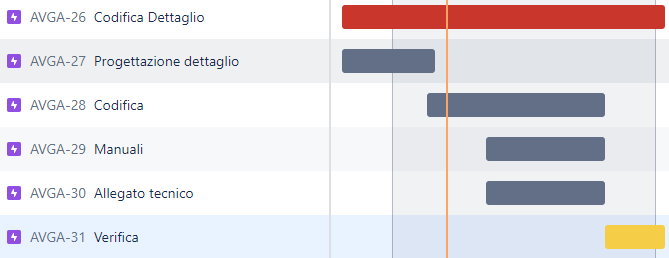
\includegraphics[width=0.75\textwidth]{images/gantt_dettaglio.PNG}
    \caption{Diagramma di Gantt della fase di codifica finale}
    \label{fig:gantt_codRTB}
\end{figure}

%%%%%%%%%%%%%%%%%%%%%%%%%%%%%%%%%%%   VALIDAZIONE   %%%%%%%%%%%%%%%%%%%%%%%%%%%%%%%%%%%

\subsection{Validazione e collaudo}\label{sec:pianificazione:val_collaudo}

\textbf{Periodo}: dal 02/04/2024 al 26/04/2024\\\\
Questa fase inizia una volta completata la codifica del prodotto finale e termina con la seconda revisione. La fase è volta a verificare, revisionare e approvare il prodotto finale e la documentazione.

\subsubsection{Attività}\label{sec:pianificazione:val_collaudo:attivita}
Questa fase ha come attività principali la verifica finale ad alto livello del prodotto realizzato nella fase precedente, la validazione rispetto ai requisiti preposti e la presentazione all'azienda proponente, nonchè il completaemento e verifica finale della documentazione del progetto.

\subsubsection{Periodi}\label{sec:pianificazione:val_collaudo:periodi}
\paragraph{Primo Periodo}\label{sec:pianificazione:val_collaudo:periodi:primo}

\begin{xltabular}{\textwidth}{{0.35\textwidth} | X}
        
    \rowcolor{black}
    \textbf{\color{white} Info} & \textbf{\color{white}Primo Periodo}\\ 
    \hline
    \endhead
    
    \textbf{Data inizio} 
    & 02/04/2024 \\
    \hline

    \textbf{Data fine} 
    & 26/04/2024 \\
    \hline

    \textbf{Pre-condizione} 
    & Soddisfacimento post-condizioni del periodo precedente \\
    \hline
    
    \textbf{Post-condizione} 
    & Consegna Product Baseline \\
    \hline

    \textbf{Ruoli attivi} 
    &  \begin{itemize}
        \item Responsabile
        \item Amministratore
        \item Verificatore
    \end{itemize}\\
    \hline

    \textbf{Descrizione} 
    &  Questa fase è adibita alla verifica e validazione del codice e del completamento dei documenti prodotti durante il progetto, in vista della consegna di tutto per la terza revisione. \\
    \hline

\caption{Tabella descrittiva del periodo di verifica e validazione}\label{tab:periodo5_1}
\end{xltabular}

\subsubsection{Diagramma di Gantt}\label{sec:pianificazione:val_collaudo:gantt}

\begin{figure}[H]
    \centering
    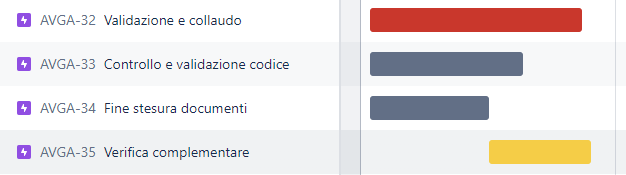
\includegraphics[width=0.75\textwidth]{images/gantt_collaudo.PNG}
    \caption{Diagramma di Gantt del periodo di verifica e validazione}
    \label{fig:gantt_collaudo}
\end{figure}

\newpage
%%%%%%%%%%%%%%%%%%%%%%%%%%%%%%%%%%%
% PREVENTIVO
%%%%%%%%%%%%%%%%%%%%%%%%%%%%%%%%%%%

\section{Preventivo}\label{sec:preventivo}

Questa sezione descrive un prospetto economico e orario del progetto, suddiviso per fasi e ruoli. Per ogni fase viene riportato ogni membro del gruppo, con le ore da esso ricoperte per ogni ruolo e infine il costo complessivo della fase per ruolo.
Ogni membro del gruppo deve ricoprire ogni ruolo almeno una volta per la durata del progetto, perciò i ruoli vengono cambiati periodicamente accordandosi con gli altri membri in modo da soddisfare questa richiesta.
Per una descrizione più dettagliata della suddivisione dei membri e dello scopo dei vari ruoli, consultare il documento \textit{Norme di Progetto} nella sezione dedicata ai processi organizzativi.\\

\subsection{Dettaglio per periodo}\label{sec:preventivo:periodi}
A seguire sono elencate tutte le fasi del progetto, con i relativi ruoli e le ore che ogni membro del gruppo dovrà ricoprire per ogni fase, seguito dal costo complessivo per fase. Per ottimizare l'utilizzo dello spazio, i vari ruoli vengono abbreviati nel modo seguente:\\
\begin{itemize}
    \item \textbf{Re:} \textit{Responsabile}
    \item \textbf{Am:} \textit{Amministratore}
    \item \textbf{An:} \textit{Analista}
    \item \textbf{Pt:} \textit{Progettista}
    \item \textbf{Pr:} \textit{Programmatore}
    \item \textbf{Ve:} \textit{Verificatore}
\end{itemize}

%%%%%%%%%%%%%%%%%%%%%%%%%%%%%%%%%%%   ANALISI   %%%%%%%%%%%%%%%%%%%%%%%%%%%%%%%%%%%

%\newpage
\subsubsection{Analisi}\label{sec:preventivo:periodi:analisi}

\begin{center}
\begin{xltabular}{\textwidth}{| 1 | {0.35\textwidth} | {0.35\textwidth} | {0.35\textwidth} | {0.35\textwidth} | {0.35\textwidth} | {0.35\textwidth} | 1 |}
        
    \rowcolor{black}
    \textbf{\color{white} Nominativo} & \textbf{\color{white}Re}& \textbf{\color{white}Am}& \textbf{\color{white}An}& \textbf{\color{white}Pt}& \textbf{\color{white}Pr}& \textbf{\color{white}Ve}& \textbf{\color{white}Totale ore}\\ 
    \hline
    \endhead

    Jessica Carretta & 3 & 6 & 6 & 0 & 0 & 5 & 20 \\
    \hline
    
    Giulio Biscontin & 3 & 5 & 4 & 0 & 0 & 8 & 20 \\
    \hline
    
    Luca Securo & 2	& 0 & 10 & 0 & 0 & 8 & 20 \\
    \hline
    
    Andrea Mangolini & 5 &	6 &	4 &	0 &	0 &	5 &	20 \\
    \hline
    
    Zaccaria Marangon & 2 & 0 & 5 & 0 & 0 & 13 & 20 \\
    \hline
    
    Lorenzo Pasqualotto & 4 & 4 & 9 & 0 & 0 & 3 & 20 \\
    \hline

\caption{Suddivisione dei ruoli nel periodo di Analisi Preliminare}\label{tab:ruoli_analisi}
\end{xltabular}
\end{center}

\begin{center}
\begin{xltabular}{\textwidth}{| 1 | {0.35\textwidth} | 1 |}
            
    \rowcolor{black}
    \textbf{\color{white} Ruolo} & \textbf{\color{white} Ore} & \textbf{\color{white} Costo}\\ 
    \hline
    \endhead

    Responsabile & 19 & €570,00 \\
    \hline
    
    Amministratore & 21 & €420,00 \\
    \hline
    
    Analista & 38 & €950,00 \\
    \hline
    
    Progettista & 0 & €0,00 \\
    \hline
    
    Programmatore & 0 & €0,00 \\
    \hline
    
    Verificatore & 42 & €630,00 \\
    \hline
    
    \textbf{Totale} & \textbf{120} & \textbf{€2.570,00} \\
    \hline
        
    \caption{Costo per ruolo Analisi Preliminare}\label{tab:costo_analisi}
\end{xltabular}
\end{center}

\begin{figure}[H]
    \centering
    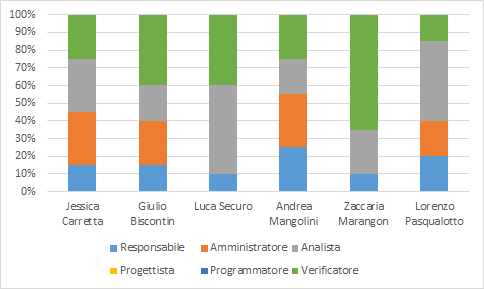
\includegraphics[width=0.75\textwidth]{images/grafico_analisi.png}
    \caption{Grafico a barre suddivisione ruoli Analisi Preliminare}
    \label{fig:grafico_analisi}
\end{figure}

\begin{figure}[H]
    \centering
    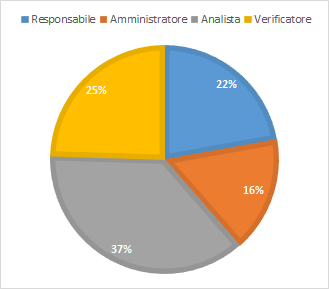
\includegraphics[width=0.5\textwidth]{images/torta_analisi.png}
    \caption{Grafico a torta suddivisione costi per ruolo Analisi Preliminare}
    \label{fig:torta_analisi}
\end{figure}

%%%%%%%%%%%%%%%%%%%%%%%%%%%%%%%%%%%   PROGETTAZIONE RTB   %%%%%%%%%%%%%%%%%%%%%%%%%%%%%%%%%%%

\newpage
\subsubsection{Realizzazione Proof of Concept}\label{sec:preventivo:periodi:progRTB}

\begin{center}
\begin{xltabular}{\textwidth}{| 1 | {0.35\textwidth} | {0.35\textwidth} | {0.35\textwidth} | {0.35\textwidth} | {0.35\textwidth} | {0.35\textwidth} | 1 |}
        
    \rowcolor{black}
    \textbf{\color{white} Nominativo} & \textbf{\color{white}Re}& \textbf{\color{white}Am}& \textbf{\color{white}An}& \textbf{\color{white}Pt}& \textbf{\color{white}Pr}& \textbf{\color{white}Ve}& \textbf{\color{white}Totale ore}\\ 
    \hline
    \endhead

    Jessica Carretta & 4 & 3 & 3 & 8 & 7 & 7 & 32 \\
    \hline
    
    Giulio Biscontin & 2 & 0 & 4 & 5 & 13 & 8 & 32 \\
    \hline
    
    Luca Securo & 3	& 6 & 0 & 7 & 10 & 6 & 32 \\
    \hline
    
    Andrea Mangolini & 2 &	1 &	0 &	8 & 11 & 10 & 32 \\
    \hline
    
    Zaccaria Marangon & 2 & 4 & 2 & 6 & 10 & 8 & 32 \\
    \hline
    
    Lorenzo Pasqualotto & 1 & 4 & 0 & 2 & 10 & 15 & 32 \\
    \hline

\caption{Suddivisione dei ruoli nel periodo di Realizzazione Proof of Concept}\label{tab:ruoli_progRTB}
\end{xltabular}
\end{center}

\begin{center}
\begin{xltabular}{\textwidth}{| 1 | {0.35\textwidth} | 1 |}
            
    \rowcolor{black}
    \textbf{\color{white} Ruolo} & \textbf{\color{white} Ore} & \textbf{\color{white} Costo}\\ 
    \hline
    \endhead

    Responsabile & 14 & €420,00 \\
    \hline
    
    Amministratore & 18 & €360,00 \\
    \hline
    
    Analista & 9 & €225,00 \\
    \hline
    
    Progettista & 36 & €900,00 \\
    \hline
    
    Programmatore & 61 & €915,00 \\
    \hline
    
    Verificatore & 54 & €810,00 \\
    \hline
    
    \textbf{Totale} & \textbf{192} & \textbf{€3.630,00} \\
    \hline
        
    \caption{Costo per ruolo realizzazione Proof of Concept}\label{tab:costo_progRTB}
\end{xltabular}
\end{center}

\begin{figure}[H]
    \centering
    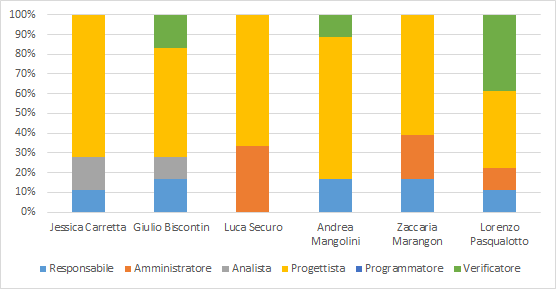
\includegraphics[width=0.75\textwidth]{images/grafico_progPOC.png}
    \caption{Grafico a barre suddivisione ruoli realizzazione RTB}
    \label{fig:grafico_progRTB}
\end{figure}

\begin{figure}[H]
    \centering
    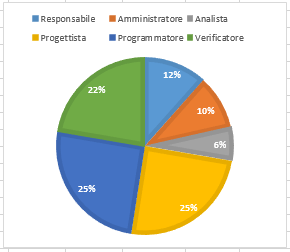
\includegraphics[width=0.5\textwidth]{images/torta_progPOC.png}
    \caption{Grafico a torta suddivisione costi per ruolo realizzazione RTB}
    \label{fig:torta_progRTB}
\end{figure}

%%%%%%%%%%%%%%%%%%%%%%%%%%%%%%%%%%%   CODIFICA DETTAGLIO   %%%%%%%%%%%%%%%%%%%%%%%%%%%%%%%%%%%

%\newpage
\subsubsection{Progettazione dettaglio e codifica}\label{sec:preventivo:periodi:dettaglio}

\begin{center}
    \begin{xltabular}{\textwidth}{| 1 | {0.35\textwidth} | {0.35\textwidth} | {0.35\textwidth} | {0.35\textwidth} | {0.35\textwidth} | {0.35\textwidth} | 1 |}
            
        \rowcolor{black}
        \textbf{\color{white} Nominativo} & \textbf{\color{white}Re}& \textbf{\color{white}Am}& \textbf{\color{white}An}& \textbf{\color{white}Pt}& \textbf{\color{white}Pr}& \textbf{\color{white}Ve}& \textbf{\color{white}Totale ore}\\ 
        \hline
        \endhead
    
        Jessica Carretta & 2 & 0 & 0 & 9 & 18 & 5 & 34 \\
        \hline
        
        Giulio Biscontin & 5 & 1 & 0 & 11 & 11 & 6 & 34 \\
        \hline
        
        Luca Securo & 3	& 0 & 0 & 10 & 13 & 8 & 34 \\
        \hline
        
        Andrea Mangolini & 2 &	0 &	4 &	10 & 13 & 5 & 34 \\
        \hline
        
        Zaccaria Marangon & 2 & 5 & 0 & 12 & 15 & 0 & 34 \\
        \hline
        
        Lorenzo Pasqualotto & 5 & 0 & 0 & 15 & 14 & 0 & 34 \\
        \hline
    
    \caption{Suddivisione dei ruoli nel periodo di progettazione e codifica dettaglio}\label{tab:ruoli_dettaglio}
    \end{xltabular}
\end{center}

\begin{center}
\begin{xltabular}{\textwidth}{| 1 | {0.35\textwidth} | 1 |}
            
    \rowcolor{black}
    \textbf{\color{white} Ruolo} & \textbf{\color{white} Ore} & \textbf{\color{white} Costo}\\ 
    \hline
    \endhead

    Responsabile & 13 & €390,00 \\
    \hline
    
    Amministratore & 6 & €120,00 \\
    \hline
    
    Analista & 4 & €100,00 \\
    \hline
    
    Progettista & 67 & €1.675,00 \\
    \hline
    
    Programmatore & 84 & €1.260,00 \\
    \hline
    
    Verificatore & 24 & €360,00 \\
    \hline
    
    \textbf{Totale} & \textbf{198} & \textbf{€3.855,00} \\
    \hline
        
    \caption{Costo per ruolo progettazione e codifica dettaglio}\label{tab:costo_dettaglio}
\end{xltabular}
\end{center}

\begin{figure}[H]
    \centering
    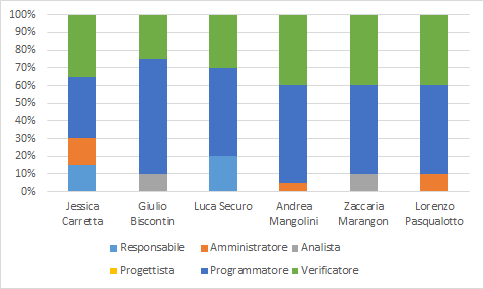
\includegraphics[width=0.75\textwidth]{images/grafico_codPOC.png}
    \caption{Grafico a barre suddivisione ruoli progettazione e codifica dettaglio}
    \label{fig:grafico_dettaglio}
\end{figure}

\begin{figure}[H]
    \centering
    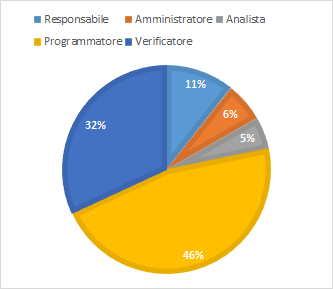
\includegraphics[width=0.5\textwidth]{images/torta_codPOC.png}
    \caption{Grafico a torta suddivisione costi per ruolo progettazione e codifica dettaglio}
    \label{fig:torta_dettaglio}
\end{figure}

%%%%%%%%%%%%%%%%%%%%%%%%%%%%%%%%%%%   VALIDAZIONE   %%%%%%%%%%%%%%%%%%%%%%%%%%%%%%%%%%%

%\newpage
\subsubsection{Verifica e collaudo}\label{sec:preventivo:periodi:collaudo}

\begin{center}
    \begin{xltabular}{\textwidth}{| 1 | {0.35\textwidth} | {0.35\textwidth} | {0.35\textwidth} | {0.35\textwidth} | {0.35\textwidth} | {0.35\textwidth} | 1 |}
            
        \rowcolor{black}
        \textbf{\color{white} Nominativo} & \textbf{\color{white}Re}& \textbf{\color{white}Am}& \textbf{\color{white}An}& \textbf{\color{white}Pt}& \textbf{\color{white}Pr}& \textbf{\color{white}Ve}& \textbf{\color{white}Totale ore}\\ 
        \hline
        \endhead
    
        Jessica Carretta & 0 & 0 & 0 & 0 & 0 & 8 & 8 \\
        \hline
        
        Giulio Biscontin & 0 & 2 & 0 & 0 & 0 & 6 & 8 \\
        \hline
        
        Luca Securo & 0 & 3 & 0 & 0 & 0 & 5 & 8 \\
        \hline
        
        Andrea Mangolini & 2 & 0 & 0 & 0 & 0 & 6 & 8 \\
        \hline
        
        Zaccaria Marangon & 5 & 0 & 0 & 0 & 0 & 3 & 8 \\
        \hline
        
        Lorenzo Pasqualotto & 0 & 0 & 0 & 0 & 0 & 8 & 8 \\
        \hline
    
    \caption{Suddivisione dei ruoli nel periodo di verifica e collaudo}\label{tab:ruoli_collaudo}
    \end{xltabular}
\end{center}

\begin{center}
\begin{xltabular}{\textwidth}{| 1 | {0.35\textwidth} | 1 |}
            
    \rowcolor{black}
    \textbf{\color{white} Ruolo} & \textbf{\color{white} Ore} & \textbf{\color{white} Costo}\\ 
    \hline
    \endhead

    Responsabile & 7 & €210,00 \\
    \hline
    
    Amministratore & 5 & €100,00 \\
    \hline
    
    Analista & 0 & €0,00 \\
    \hline
    
    Progettista & 0 & €0,00 \\
    \hline
    
    Programmatore & 0 & €0,00 \\
    \hline
    
    Verificatore & 36 & €540,00 \\
    \hline
    
    \textbf{Totale} & \textbf{48} & \textbf{€850,00} \\
    \hline
        
    \caption{Costo per ruolo verifica e collaudo}\label{tab:costo_collaudo}
\end{xltabular}
\end{center}

\begin{figure}[H]
    \centering
    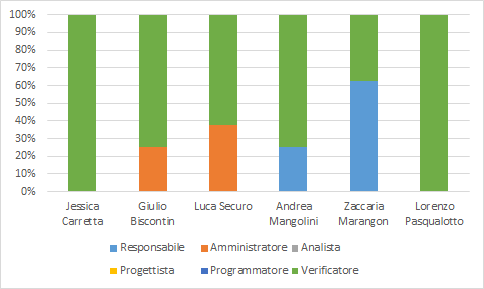
\includegraphics[width=0.75\textwidth]{images/grafico_collaudo.png}
    \caption{Grafico a barre suddivisione ruoli verifica e collaudo}
    \label{fig:grafico_collaudo}
\end{figure}

\begin{figure}[H]
    \centering
    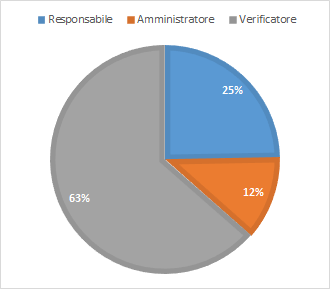
\includegraphics[width=0.5\textwidth]{images/torta_collaudo.png}
    \caption{Grafico a torta suddivisione costi per ruolo verifica e collaudo}
    \label{fig:torta_collaudo}
\end{figure}

\subsection{Prospetto economico e prospetto orario complessivi}\label{sec:preventivo:totale}
Per queste voci si rimanda al documento \textit{Suddivisione dei ruoli e preventivo dei  costi}, presente alla sezione ``Candidatura'' del \href{https://avant-garde-software-engineering.github.io/documentazione.html}{repository documentale del gruppo}.



\newpage
%%%%%%%%%%%%%%%%%%%%%%%%%%%%%%%%%%%
% CONSUNTIVO DI PERIODO
%%%%%%%%%%%%%%%%%%%%%%%%%%%%%%%%%%%
\section{Consuntivo di periodo}\label{sec:consuntivo}

Di seguito viene presentato un consuntivo per i diversi periodi del progetto, in cui si confrontano le ore preventivate con quelle effettivamente impiegate e i costi preventivati con quelli effettivi, nonchè le difficoltate incontrate e le strategie utilizzaate per mitigare i rischi.\\

\subsection{Analisi}\label{sec:consuntivo:analisi}

\begin{center}
    \textbf{Data inizio:} 06/11/2023 \\
    \textbf{Data fine:} 06/01/2024 \\
    \begin{xltabular}{\textwidth}{| 1 | 1 | {0.35\textwidth} | 1 | 1 |}
                
        \rowcolor{black}
        \textbf{\color{white} Ruolo} & \textbf{\color{white} Totale ore} & \textbf{\color{white} Diff. ore} & \textbf{\color{white} Totale costo} & \textbf{\color{white} Diff. costo}\\ 
        \endhead
    
        Responsabile & 19 & 0 & €570,00 & €0,00 \\
        \hline
        
        Amministratore & 25 & +4 & €500,00 & +€80,00 \\
        \hline
        
        Analista & 42 & +4 & €1050,00 & +€100,00 \\
        \hline
        
        Progettista & 0 & 0 & €0,00 & €0,00 \\
        \hline
        
        Programmatore & 0 & 0 & €0,00 & €0,00 \\
        \hline
        
        Verificatore & 36 & -6 & €540,00 & -€90,00 \\
        \hline
        
        \textbf{Totale} & \textbf{122} & \textbf{+2} & \textbf{€2.660,00} & \textbf{+€90,00} \\
        \hline
            
        \caption{Differenza ore e costi previsti con effettivi, Analisi}\label{tab:consuntivo_analisi}
    \end{xltabular}
\end{center}

\subsubsection{Resoconto periodo}\label{sec:consuntivo:analisi:resoconto}

Dal consuntivo di periodo emerge che il gruppo è stato in generale abbastanza in linea con il preventivo,
 con un leggero aumento dei costi dovuto alle ore aggiuntive impiegate dai ruoli di amministratore ed analista.
Questo aumento è stato causato da una sottostima delle ore necessarie per la stesura dei documenti,
 in quanto era per noi la prima esperienza in questo ambito e si è rivelato più dispendioso in termini di tempo di quanto ci aspettassimo.
Inoltre, l'analisi dei requisiti è stata più complessa del previsto, in quanto il capitolato richiedeva una buona comprensione
 del dominio applicativo e abbiamo dovuto effettuare ricerche approfondite nell'ambito.\\
Nonostante ciò, il gruppo è riuscito a rispettare i tempi di consegna e a mantenere i costi entro i limiti previsti, grazie ad una buona organizzazione
 e ad un lavoro costante e collaborativo, perciò non sono previsti cambiamenti per il prossimo periodo.\\

\newpage
\subsubsection{Mitigazione rischi attuata}\label{sec:consuntivo:analisi:mitigazione}

A seguito vengono riportati alcuni rischi incontrati e la metigazione effettuata per tali rischi.\\

\paragraph{Rischi organizzativi}

\begin{center}


    \begin{xltabular}{\textwidth}{| X | X |}
                
        \rowcolor{black}
        \textbf{\color{white} Descrizione} & \textbf{\color{white} Mitigazione}\\ 
        \endhead
    
        A causa dei diversi impegni di ogni componente del gruppo, gli orari di disponibilità offerti dagli individui erano spesso molto diversi tra loro &
        Sono stati utilizzati efficientemente i mezzi di comunicazione specificati nelle norme di progetto e il gruppo si è suddiviso i compiti dividendosi in gruppi più piccoli
        con simili disponibilità orarie \\
        \hline
            
        \caption{Tabella descrittiva rischi organizzativi e mitigazioni periodo Analisi}\label{tab:rischi_organizzativi_analisi}
    \end{xltabular}
\end{center}

\paragraph{Rischi tecnologici}

\begin{center}
    \begin{xltabular}{\textwidth}{| X | X |}
                
        \rowcolor{black}
        \textbf{\color{white} Descrizione} & \textbf{\color{white} Mitigazione}\\ 
        \endhead
    
        Essendo molte delle tecnologie utilizzate nuove per il gruppo, era presente il rischio di non riuscire ad utilizzare al meglio tali strumenti &
        Dopo aver osservato tutti i lati positivi e negativi delle opzioni per le tecnologie, il gruppo ha scelto quelle più adatte e comode e ne ha effettuato uno studio
        per poterle utilizzare al meglio. \\
        \hline
            
        \caption{Tabella descrittiva rischi tecnologici e mitigazioni periodo Analisi}\label{tab:rischi_tecnologici_analisi}
    \end{xltabular}
\end{center}

\subsection{Realizzazione Proof of Concept}\label{sec:consuntivo:progRTB}
\begin{center}
    \textbf{Data inizio:} 07/01/2024 \\
    \textbf{Data fine:} 25/03/2024 \\
    \begin{xltabular}{\textwidth}{| 1 | 1 | {0.35\textwidth} | 1 | 1 |}
                
        \rowcolor{black}
        \textbf{\color{white} Ruolo} & \textbf{\color{white} Totale ore} & \textbf{\color{white} Diff. ore} & \textbf{\color{white} Totale costo} & \textbf{\color{white} Diff. costo}\\ 
        \endhead
    
        Responsabile & 14 & 0 & €570,00 & €0,00 \\
        \hline
        
        Amministratore & 18 & 0 & €500,00 & €0,00 \\
        \hline
        
        Analista & 12 & +3 & €300,00 & +€75,00 \\
        \hline
        
        Progettista & 24 & -12 & €600,00 & -€300,00 \\
        \hline
        
        Programmatore & 70 & +9 & €1050,00 & +€135,00 \\
        \hline
        
        Verificatore & 54 & 0 & €810,00 & €0,00 \\
        \hline
        
        \textbf{Totale} & \textbf{192} & \textbf{0} & \textbf{€3.540,00} & \textbf{-€90,00} \\
        \hline
            
        \caption{Differenza ore e costi previsti con effettivi, PoC}\label{tab:consuntivo_analisi}
    \end{xltabular}
\end{center}

\subsubsection{Resoconto periodo}\label{sec:consuntivo:analisi:resoconto}

Dal consuntivo di periodo emergono alcuni problemi che sono sorti durante questo periodo. 
In particolare, il ruolo di progettista ha impiegato meno ore di quelle preventivate, in quanto il gruppo ha deciso di concentrarsi maggiormente sulla codifica
del PoC, il quale è stato codificato principalmente per testare le tecnologie utilizzate e non per creare un prodotto completo, in modo da avere una base solida
su cui basare la progettazione del prodotto finale. Inoltre, il ruolo di analista ha impiegato più ore di quelle preventivate in quanto alcune richieste presentate
 dal proponente non erano chiare e abbiamo dovuto effettuare delle modifiche al documento dell'analisi dei requisiti.\\
Dal consuntivo emerge inoltre che il gruppo ha sforato molto sul tempo di consegna previsto, in quanto il rallentamento del lavoro causato dagli esami universitari
ha portato ad un ritardo nella consegna del PoC, e una incorretta valutazione delle tecnologie sufficienti per la realizzazione del PoC ha portato ad uno sforo dei
tempi preventivati di consegna del PoC, in quanto implementare tecnologie aggiuntive ha richiesto la ricostruzione della maggior parte del codice.\\
Su queste basi, il gruppo ha deciso di effettuare sostanziali modifiche alla pianificazione dei periodi successivi, in modo da recuperare il ritardo accumulato,
prestando più attenzione a ciò che il gruppo ha deciso, assicurandoci di seguire strettamente le scelte illustrate nei documenti realizzati e coordinando in maniera
più efficiente i vari membri in base alle proprie disponibilità e capacità.\\


\subsubsection{Mitigazione rischi attuata}\label{sec:consuntivo:analisi:mitigazione}

A seguito vengono riportati alcuni rischi incontrati e la metigazione effettuata per tali rischi.\\

\paragraph{Rischi organizzativi}

\begin{center}


    \begin{xltabular}{\textwidth}{| X | X |}
                
        \rowcolor{black}
        \textbf{\color{white} Descrizione} & \textbf{\color{white} Mitigazione}\\ 
        \endhead
    
        A causa della sessione invernale degli esami universitari, il tempo disponibile offerto dal gruppo per lavorare nel progetto era minimo. &
        Il gruppo si impegna a non arrestare completamente il lavoro che viene svolto durante gli esami e dedica una quantità di tempo ogni giorno
        all'avanzamento sul progetto, in modo da poter ritornare a ritmo normale più facilmente una volta finiti gli esami \\
        \hline
            
        \caption{Tabella descrittiva rischi organizzativi e mitigazioni periodo Analisi}\label{tab:rischi_organizzativi_poc}
    \end{xltabular}
\end{center}

\paragraph{Rischi tecnologici}

\begin{center}
    \begin{xltabular}{\textwidth}{| X | X |}
                
        \rowcolor{black}
        \textbf{\color{white} Descrizione} & \textbf{\color{white} Mitigazione}\\ 
        \endhead
    
        Le tecnologie utilizzate nel progetto sconosciute e con limitata documentazione &
        I membri del gruppo si impegnano non solo a studiare singolarmente le tecnologie scelte, ma anche a condividere con il resto del team ciò che imparano
        tramite la scrittura del codice \\
        \hline
            
        \caption{Tabella descrittiva rischi tecnologici e mitigazioni periodo Proof of Concept}\label{tab:rischi_tecnologici_poc}
    \end{xltabular}
\end{center}

\newpage
%%%%%%%%%%%%%%%%%%%%%%%%%%%%%%%%%%%
% MITIGAZIONE DEI RISCHI
%%%%%%%%%%%%%%%%%%%%%%%%%%%%%%%%%%%
%\section{Difficoltà incontrate e mitigazione dei rischi}\label{sec:mitigazione_rischi}
% Scrivere le soluzioni implementate per risolvere i problemi derivanti da rischi effettivamente riscontrati
% DA SCRIVERE UNA VOLTA CHE SI SONO EFFETTIVAMENTE VERIFICATI DEI RISCHI


\newpage
%%%%%%%%%%%%%%%%%%%%%%%%%%%%%%%%%%%
% RIFERIMENTI ESTERNI
%%%%%%%%%%%%%%%%%%%%%%%%%%%%%%%%%%%
\newpage
\section{Riferimenti esterni}\label{sec:riferimenti_esterni}
Per ulteriori chiarimenti sugli argomenti discussi nel documento, si possono consultare i seguenti link esterni:
\begin{itemize}
    \item Capitolato \textbf{Warehouse Management 3D}:\\
    \url{https://www.math.unipd.it/~tullio/IS-1/2023/Progetto/C5.pdf}
    \item Link alla \textbf{documentazione del gruppo}:\\
    \url{https://avant-garde-software-engineering.github.io/documentazione.html}
    \item Link alle \textbf{slides sul ciclo di vita del software}:\\
    \url{https://www.math.unipd.it/~tullio/IS-1/2023/Dispense/T3.pdf}
    \item Link alle \textbf{slides sulla gestione di progetto}:\\
    \url{https://www.math.unipd.it/~tullio/IS-1/2023/Dispense/T4.pdf}   
\end{itemize}